\documentclass[UTF8]{ctexart}
\usepackage{amsmath}
\usepackage{xfrac}
\usepackage{graphicx}
\usepackage{float}
\usepackage{listings}
\lstset{language=Matlab}

\title{动态规划求解DELS问题}
\author{U201715825 \quad 管实-江诗毅}
\date{\today}

\begin{document}
\maketitle
\tableofcontents


\begin{abstract}
	首先给出了动态规划的一般形式,建立时间复杂度为\(O(n^2)\)一般算法,然后由任务3启发,实现了时间复杂度为\(O(n)\)的特殊动态规划算法。

	之后,使用算例拟合算法的时间复杂度,验证它们分别符合\(O(n^2)\),以及\( O(n) \)。
	
	然后给出了算法实现的思路。并对比了两种算法的区别。
	
	然后给出了验证算法正确性的测试用例。
	
	最后总结收获。
\end{abstract}
\textbf{关键词:} 动态规划

\section{从前往后的动态规划}
\subsection{更改定义}
为了方便计算,修改了从后往前的动态规划形式,将其改为了从千万后的形式,这与原问题是等价的。

project1中的其他参数定义不变,只修改\( g() \)的定义,将动态规划形式改为
\[ g(n) = \min_{m}\{ g(m) + l(m,n+1) : 1 \leq m < n \leq N \}, n = 1,2,\cdots N \]

这与project1中的表达式表意相同,但是方便了问题的分析。
\subsection{验证\( O(n^2) \)时间复杂度}
根据时间复杂度为\( O(n^2) \)的算法,后面会解释原因。绘制出时间随规模变化的曲线。(图1,图2)

稀疏点拟合的参数分别为\(a=0.0000\cdot 10^{-4}\quad b=-0.0058\cdot 10^{-4}\quad c=0.1412\cdot 10^{-4}\)

密集点拟合的参数分别为\(a=0.0000\cdot 10^{-4}\quad b=-0.0065\cdot 10^{-4}\quad c=0.1921\cdot 10^{-4}\)

\begin{figure}[H] %[htbp]
	\centering
	\begin{minipage}[t]{1\textwidth}
		\centering
		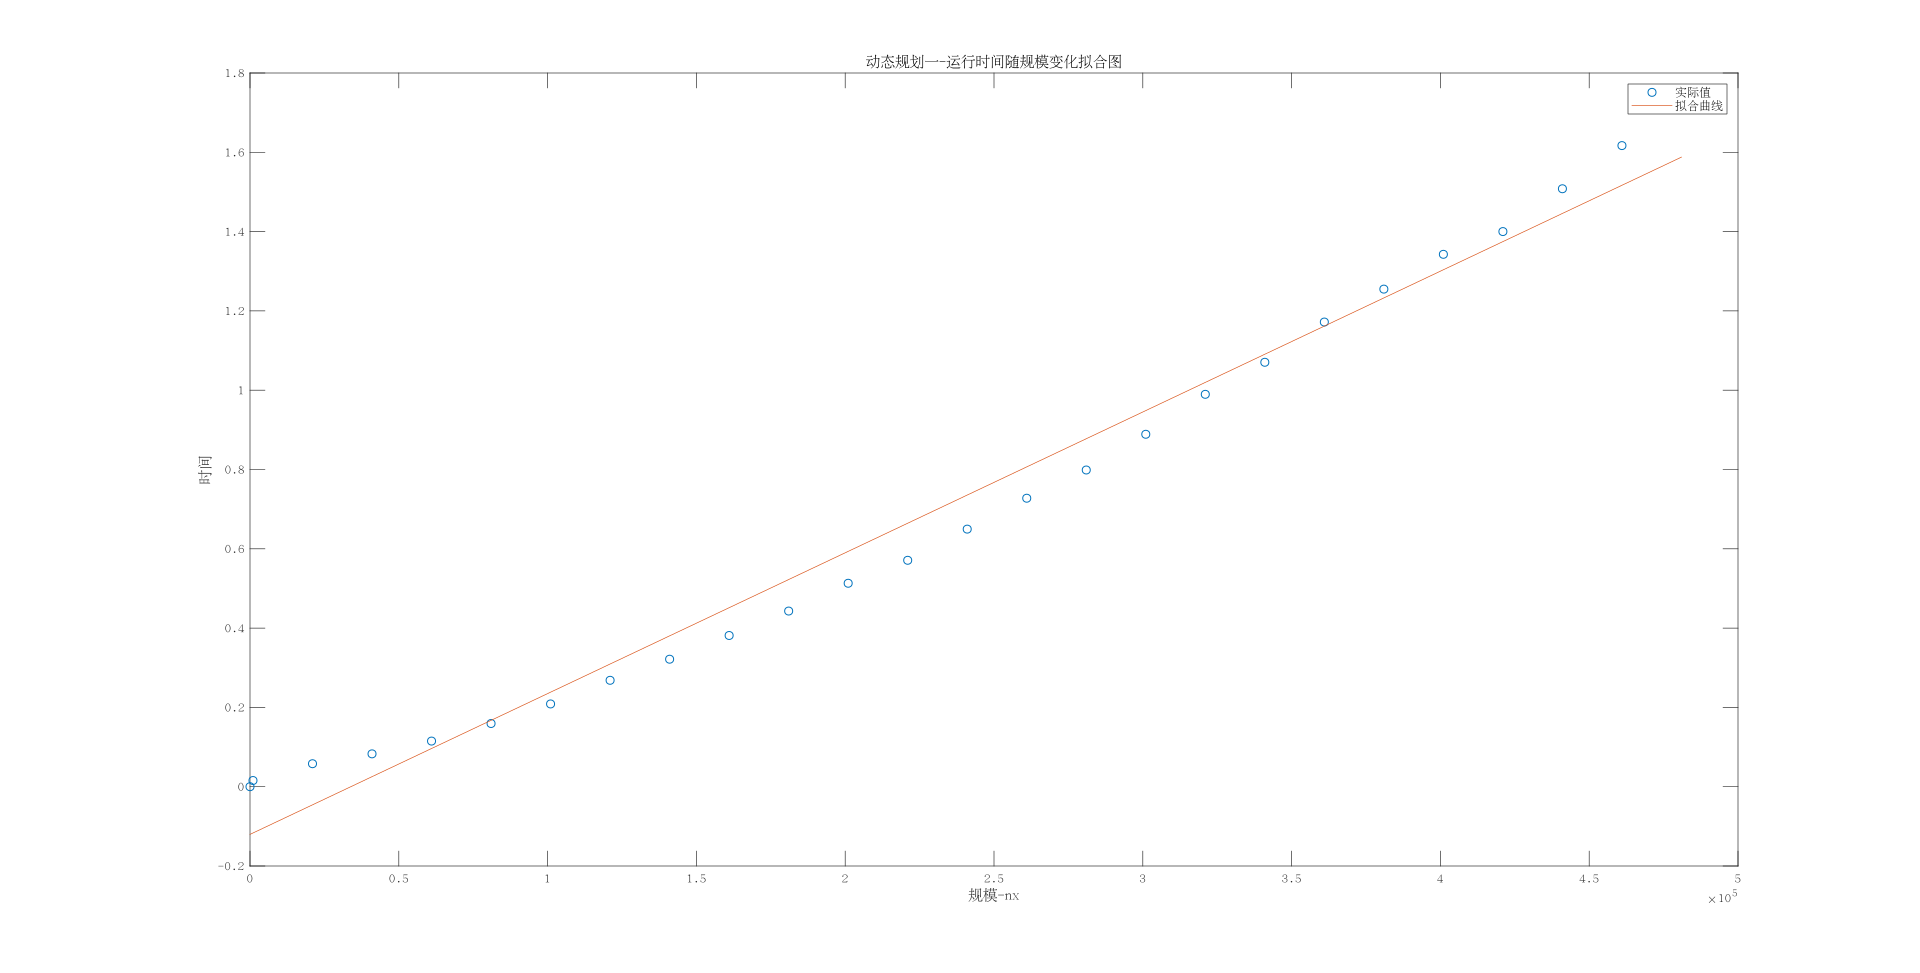
\includegraphics[width=12cm]{1.jpg}
		\caption{稀疏点拟合}
	\end{minipage}
	\begin{minipage}[t]{1\textwidth}
		\centering
		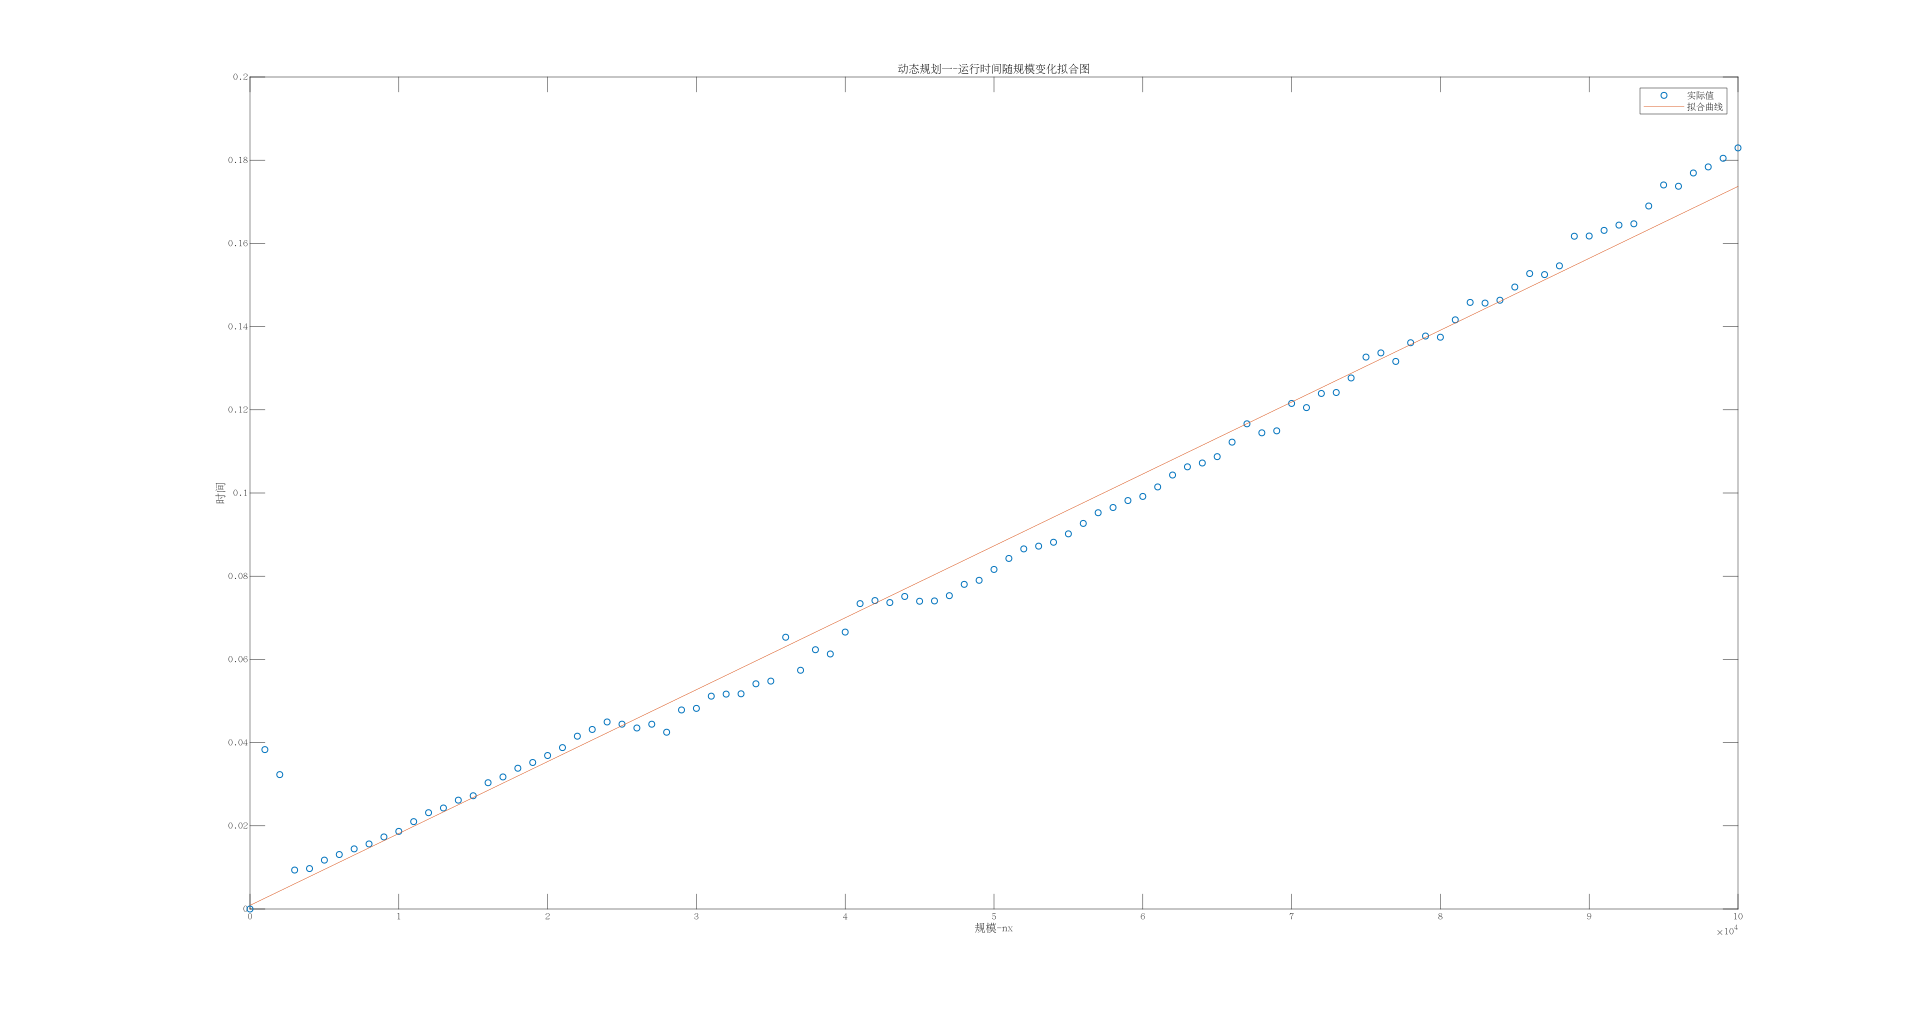
\includegraphics[width=12cm]{2.jpg}
		\caption{密集点拟合}
	\end{minipage}
\end{figure}

\subsection{验证\( O(n) \)时间复杂度}
根据时间复杂度为\( O(n) \)的算法,后面会解释原因,绘制出时间随规模变化的曲线。(图3,图4)

稀疏点拟合的参数分别为\(k=0.1223 \cdot 10^{-4}\)

密集点拟合的参数分别为\(k=0.6295 \cdot 10^{-4}\)

\begin{figure}[H]                 
	\centering
	\begin{minipage}[t]{1\textwidth}
		\centering
		\includegraphics[width=12cm]{3.jpg}
		\caption{稀疏点拟合}
	\end{minipage}
	\begin{minipage}[t]{1\textwidth}
		\centering
		\includegraphics[width=12cm]{4.jpg}
		\caption{密集点拟合}
	\end{minipage}
\end{figure}

\subsection{误差分析}
使用上图中任一结果,分析其均方误差。\( MSE = 0.00023 \)

数据来源如下图5(每一项的误差值)。可知拟合的结果较好,所以不拒绝两个算法复杂度分别为\( O(n^2),O(n) \).

\begin{figure}[H]
	\centering
	\includegraphics[width=1\linewidth]{../../../../../图片/选区_196}
	\caption{}
	\label{fig:196}
\end{figure}

\section{实现思路}
将该问题分解成各个小问题,逐一解决,模块化代码,最后给出结论。

\subsection{计算m期生产满足到第n-1期的成本}
~\\
\textbf{确定子程序输入输出},具体代码见mToNCost.m附件
\begin{lstlisting}
%
%输入:
%   d(vector) : 各阶段的需求
%   k(vector) : 各阶段的固定成本
%   c(vector) : 各阶段的单位边际成本
%   h(vector) : 各阶段的持有库存的边际成本
%   m(number) : 开始的阶段
%   n(number) : 结束的后一阶段
%
%输出:
%   cost(number) : 第m期生产满足第m到n-1期的所有需求带来的成本
\end{lstlisting}

~\\
\textbf{第一种实现方式}
\begin{lstlisting}
% 计算m期生产的成本
cost = k(m) + c(m) * sum(d(m:n-1));
% 累计从m 到 n-1期的 所有 holding cost 
for i=m  to  n-2
    cost +=  h(i) .* sum(d(i+1:n-1));
\end{lstlisting}

~\\
\textbf{第二种实现方式}

给出\( c_{m,i} \)表达式
\[ c_{m,i} = c_m + h_m + \cdots + h_{i-1} \]


~\\
\textbf{第三种实现方式}

更改\( l_{m,n} \)表达式
\[ l(m,n) = k_m + c_{m,N+1}d_{1,n+1} \]

经过验证,可知它不符合问题的描述,且计算出的成本会增大很多。


\subsection{计算最低成本}
\textbf{功能描述}
\begin{lstlisting}
%算法时间复杂度为O(n^2),n为维度
%输入:
%   d(vector) : 各阶段的需求
%   k(vector) : 各阶段的固定成本
%   c(vector) : 各阶段的单位边际成本
%   h(vector) : 各阶段的持有库存的边际成本
%
%输出:
%   result(number) : 最小成本
%   road(vector) : 达到最小成本的方案(0代表不生产,1代表生产)
%
%example(d,k,c,h都为n维向量):
%   [optResult,road] = dySolution(d,k,c,h)
\end{lstlisting}


\textbf{思路},matlab代码见dySolution.m附件。

步骤:
\begin{itemize}
    \item 基本的输入向量验证,例如 验证维度是否符合要求。
    \item 预分配内存,提高效率:一维数组r表示从第1期到第n期的最小成本,该问题是动态规划的子问题。一维数组s表示r(n)对应最优子方案中最后一次生产的时期是在第s(n)阶段。
    \item 迭代求解子问题,例如现在是第i次循环,依次遍历s(i)= 1 to i,计算值,记录下最优路线方案,以及最有成本。
    \item 重复步骤3,直到r(n)被算出,停止迭代。
\end{itemize}

\subsection{计算最优路线}
根据2.2小节给出的s(n) 的定义,可以迭代出每个子问题对应的最优决策方案。

\textbf{思路},matlab代码将dyRoad.m附件

步骤:
\begin{itemize}
    \item 路径的递归定义: 1 ---> ... ---> s(s(n) - 1) --->  s(n) ---> N 
    \item 从s(n)开始,表示最后生产的阶段。
    \item 继续计算s( s(n)-1 ),表示倒数第二次的生产阶段。
    \item 重复下去,直到回到s(i) - 1 < 0。 
\end{itemize}

\subsection{检查一个路线是否是最优路线}
由于对于每组d,k,c,h都有可能有多个最优解,故给出了核查给定road是否是最优方案的方法。

\textbf{思路},matlab代码见checkOptRoad.m附件
\begin{lstlisting}
%checkOptRoad - 判断给定路径是否是动态规划的最优解
%
%输入:
%   d(vector) : 各阶段的需求
%   k(vector) : 各阶段的固定成本
%   c(vector) : 各阶段的单位边际成本
%   h(vector) : 各阶段的持有库存的边际成本
%   road(vector) : 路线
%
%输出:
%   result(boolean) : 逻辑1或者逻辑0

% 根据路线给出成本
sum_cost
% 比较最优成本与sum_cost
return sum_cost == dySolution(d,k,c,h)
\end{lstlisting}

\subsection{受任务3启发,给出时间复杂度为O(n)的算法}
根据任务三,如果已经得到了第n期之后的最优生产期分别为 \( n=s_o < s_1 < s_2 < \cdots < s_m \leq N \),那么在计算第n-1期之后的最优生产计划时,\( s_0,s_1 \)可能会更新,但是\( s_2 \)及以后的计划期不会改变。

由于我是采用从前往后的算法,故我得出与之对称的猜想。如果已经得到了第m期之前的最优生产期分别为 \( n=s_o < s_1 < s_2 < \cdots < s_n \leq m \),那么在计算第m+1期之后的最优生产计划时,\( s_m,s_{m-1} \)可能会更新,但是\( s_{n-2} \)及之前的计划期不会改变。也就是说最多会改变最近两期的决策。

算例验证如下图所示,可以看出最多只有最近两期的决策会发生改变。

\begin{figure}[H]                 
    \centering
    \begin{minipage}[t]{1\textwidth}
        \centering
        \includegraphics[width=12cm]{11.png}
        \caption{稀疏点拟合}
    \end{minipage}
    \begin{minipage}[t]{1\textwidth}
        \centering
        \includegraphics[width=12cm]{../../../../../图片/选区_197}
        \caption{密集点拟合}
    \end{minipage}
\end{figure}


\textbf{实现思路}

步骤:
\begin{itemize}
    \item 先计算出第一期,以及第一期到第二期的最优决策值。
    \item 从第三期开始迭代,每次只用分四种情况计算最优值。1. 最近的两期都不生产。2. 最近的二期生产,最近的一期不生产。3. 最近的一期不生产,最近的二期生产。 4. 最近的两期都生产。
    \item 比较上面四个结果,得出最优值以及方案。
\end{itemize}

可以得出结论,在该特殊动态规划中,在计算更大一级的问题时,比其小两级的子问题的最优路线不会发生改变,这样就不用重复计算比较选择那个子问题。相当于所有阶段只计算了一次,算法的复杂度变为O(n).


\subsection{分析两种算法的区别}
对于第一种算法,在每次子问题的迭代过程中,都要计算i-1种方案进行对比,但是在第二种算法中,只需要对比4种方案,这样算法的时间复杂度大大下降了。

在内存消耗上,都使用了两个一维数组存储问题的最优解以及最优解对应的最后一阶段期,所以两者无较大差异。

总的来说,在问题规模较小时,两种算法都较可行,但是当问题规模较大时,第二种\(O(n)\)的算法明显有优势。



\section{测试}
遵循TDD(测试驱动开发)原则,先给出代码的测试用例,然后实现算法。

\subsection{测试主程序}
主程序分别见dySolution.m(\(O(n^2)\)时间复杂度)\quad OnDySolution.m(\(O(n)\)时间复杂度)

\begin{tabular}{c c c}
	\hline
	测试用例 & 结果 & 要求 \\
	dySolution(1,1,1,1) & 通过 & 结果为2 \\
	OnDySolution(1,1,1,1) & 通过 & 结果为2\\
	dySolution(d,k,c,h) & 通过 & d,k保持不变,c或者h增加一个常数,最优方案不变 \\
	OnDySolution(d,k,c,h) & 通过 & d,k保持不变,c或者h增加一个常数,最优方案不变\\	
	dySolution(d,k,c,h) & 通过 & k=0,c,h保持不变,d不影响最优决策 \\
	OnDySolution(d,k,c,h) & 通过 & k=0,c,h保持不变,d不影响最优决策\\
	\hline
\end{tabular}

~\\

\textbf{测试主程序的伪代码(任务1给出的测试方法):}
\begin{lstlisting}
% 随机生成d,k,c,h,以及c,h增加的同一个常数add
% 生成1000组测试用例
d,k,c,h,add = randi(10,1000,10);

for i = 1:1000
% 分别计算四种情况下的最优值
	[a1,b1] = dySolution(d(i,:),k(i,:),c(i,:),h(i,:));
	[a2,b2] = dySolution(d(i,:),k(i,:) + tem,c(i,:),h(i,:));
	[a3,b3] = dySolution(d(i,:),k(i,:),c(i,:) + tem,h(i,:));
	[a4,b4] = dySolution(d(i,:),k(i,:)+tem,c(i,:)+tem,h(i,:));
% 检验他们的最优决策方案是否相同
all([
	checkOptRoad(d(i,:),k(i,:),c(i,:) + tem,h(i,:),b1),
	checkOptRoad(d(i,:),k(i,:) + tem,c(i,:),h(i,:),b1),
	checkOptRoad(d(i,:),k(i,:) + tem,c(i,:)+tem,h(i,:),b1)
]) == 1

\end{lstlisting}

~\\

\textbf{测试主程序的伪代码(任务2给出的测试方法):}
\begin{lstlisting}
% 测试 k = 0时,最优决策与d无关。
d = randi(10,100,10);
k = zeros(1,10);
c = randi(10,1,10);
h = randi(10,1,10);
 
[opt,plan] = dySolution(d(1,:),k,c,h);
for i = 1:100
% 检验最优决策方案是否发生改变。
checkOptRoad(d(i,:),k,c,h,plan)
\end{lstlisting}


\section{结论}
逐步剖析问题,分解问题,实现各个子程序。然后优化代码,优化原来\(O(n^2)\)的算法,得出最优解法。

\end{document}